\lhead{\begin{tikzpicture}[remember picture, overlay]
    \node [anchor=100,inner sep=0] (imagenIZQUIERDA) at (current page header area.north){
\includegraphics[width=18cm]{img/Encabezado.PNG}};
    \end{tikzpicture}}
    \rhead{Ángeles-Hurtado}
    \rfoot{\begin{tikzpicture}[remember picture, overlay]
    \node [anchor=140,inner sep=0] (imagenDERECHA) at (current page footer area.south){
\includegraphics[width=18cm]{img/Foot.PNG}};
    \end{tikzpicture}}
    %----------------------------------------------------------------------------------------
    \lfoot{ \thepage}
    % \renewcommand{\labelenumi}{\alph{enumi}.)} 
    %----------------------------------------------------------------------------------------
    %----------------------------------------------------------------------------------------
    %	TITLE SECTION
    %----------------------------------------------------------------------------------------
    
    \setlength{\droptitle}{-5\baselineskip} % Move the title up
    \title{\textbf{Estudio de tiempos y movimientos en el ensamble de un circuito electrónico utilizando diferentes métodos para su optimización }} % Article title
    
     \author{ 
     \textsc{Ruiz Peña Nancy}\\ 
    %  Afiliación:
     \texttt{ Instituto Tecnologico de Queretaro  } \\ 
     \texttt{Instituto Nacional de Mexico } \\ 
     \texttt{Queretaro, Mexico}\\ 
     \texttt{Correo} 
     \and 
     \textsc{Ángeles-Hurtado, Luis Alberto}\\ 
    %  Afiliación:
     \texttt{ Instituto Tecnológico de Querétaro } \\ 
     \texttt{ Tecnológico Nacional de México } \\ 
     \texttt{Querétaro, México}\\ 
     \texttt{alb3rt0.ah@gmail.com} 
    }
    
    
    %----------------------------------------------------------------------------------------
    
    % \begin{document}
    
    % Print the title
    \maketitle
    \thispagestyle{fancy}
    
    %----------------------------------------------------------------------------------------
    %	ARTICLE CONTENTS
    %----------------------------------------------------------------------------------------
    
    % \section*{Resumen}
    % \textit{Palabras clave:}
    % El resumen (ancho de página) deberá contener entre 100 y 200 palabras tipo Adobe Devangari 11 puntos.
    
    \begin{abstract}
    \noindent 
    El resumen (ancho de página) deberá contener entre 100 y 200 palabras tipo Adobe Devangari 11 puntos.
    
    \end{abstract}
    % 
    % 
    \textbf{\textit{Palabras clave}}: {First keyword should be the corresponding to the research area according with the authors guide. Maximum of 6 keywords.}
    % \keywords{First keyword should be the corresponding to the research area according with the authors guide. Maximum of 6 keywords.}
    
    \section{Introducción}
    
    % El estudio de tiempos y movimientos:
    %  Ensamble: 
    % circuito electronico: 
    % El metodo de tiempos predeterminados: 
    % La optimización:
    \begin{itemize}
    \item Este trabajo se muestra la metodologia para un  el ensamble de un circuito electrico en el cual intervienen factores como organizacion, tiempo, movimientos y por supuesto una metodologia para que el analista pueda seguir un proceso que lo lleve al resultado final 
        \item El estudio de tiempos y movimientos:consiste  en el análisis de métodos, materiales y herramientas que se utilizan en la ejecución de un trabajo. Esta área de estudio abarca una amplia gama de campos, incluyendo la ingeniería industrial, la psicología organizacional, la ergonomía, la gestión de operaciones y la sociología laboral. \cite{EstudioDeTiemposMovimientos-2017}
         \item  Ensamble: es un proceso de fabricación industrial en el que una o varias piezas se unen para formar un producto final, se lleva a cabo en líneas de producción, en las que el trabajo se realiza a una velocidad constante. Los operarios se encargan de unir las piezas de forma manual o mecánica, y de realizar los ajustes necesarios para que el producto quede completo.
       \item circuito electronico: son placas que se componen de materiales semiconductores, activos y pasivos cuya operatividad va a depender del flujo de electrones (corriente o energía) para que se  genere, transmita, reciba y almacena una información determinada. Siendo  la unión de dos o más elementos que permitirán la circulación de la corriente eléctrica. Este hecho facilita el flujo de electricidad a la par de permitir el control de la misma.\cite{dorf2015circuitos}
      \item El metodo de tiempos predeterminados: Es un procedimiento utilizado para analizar cualquier operación o método manua. Consiste en descomponer la tarea en movimientos básicos necesarios para su ejecución, asignando a cada movimiento un tiempo predeterminado basado en su naturaleza y las condiciones bajo las cuales se realiza.\cite{book}
     \item El metodo de tiempos predeterminados: Es un procedimiento utilizado para analizar cualquier operación o método manua. Consiste en descomponer la tarea en movimientos básicos necesarios para su ejecución, asignando a cada movimiento un tiempo predeterminado basado en su naturaleza y las condiciones bajo las cuales se realiza.
     \item La optimización: es el proceso de encontrar la mejor solución posible para un problema específico, dadas ciertas restricciones o condiciones. Implica maximizar o minimizar una función objetivo, que representa algún tipo de medida de desempeño, beneficio o costo, sujeto a una serie de restricciones o limitaciones. En esta introducción seguiremos viendo las metodologías más usadas, como ha evolucionado, objetivos empleados en el  proyecto de ensamble de un circuito eléctrico, etc.
    \end{itemize}
    % 
    % 
    \section{Justificación}
    
    \begin{itemize}
        \item En la actualidad, los productos electrónicos de alta calidad están en constante crecimiento, las personas consumidoras buscan elementos cada vez más eficientes, lo que impulsa a las empresas a tener mejor proceso en la producción, el estudio de movimientos se vuelven importante para optimizar el ensamble de circuito electrónico, las empresas necesitan adoptar prácticas eficientes y efectivas.
        Además, en un mundo donde la tecnología avanza rápidamente, la capacidad de adaptarse y mejorar constantemente es esencial para mantenerse relevante.
        Mediante el uso de metodologías como los therbligs, las empresas pueden realizar ajustes precisos en sus procesos de ensamble para integrar nuevas tecnologías y
    responder rápidamente a las demandas cambiantes del mercado.
    A nivel local o nacional, la implementación de técnicas de estudio de tiempos y movimientos en el ensamble de circuitos electrónicos puede tener un impacto significativo en la economía y la
    competitividad de las empresas del sector.
    
    \end{itemize}
    % 
    % 
    \section{Descripción del problema}
    \begin{itemize}
        \item Afectación en la productividad debido a la mala identificación de movimientos innecesarios o insuficientes, quitándole la calidad del producto final, asindo que el operador tenga dificultades para acceder a las herramientas inmediatamente llevando a una disminucion en la eficiencia y un aumento en los ciclos 
       Requiere un enfoque sistemático que incluya la estandarización de
    procesos, el diseño ergonómico de estaciones de trabajo, la capacitación adecuada para los trabajadores y la implementación de mejoras continuas en el proceso de
    ensamble.
        \item Debe de tener Referencias científicas, URL, tesis, etc.
    \end{itemize}
    
    \textbf{*La incógnita científica es el elemento cuya solución incrementa el conocimiento científico.}
    % 
    % 
    \section{Fundamentación teórica}
    
    Es la parte medular y de mayor discusión, deberá ser la fundamentación de la hipótesis, por tanto se deberá señalar claramente la razón de la suposición y fundamentación de la misma. Únicamente referencias científicas.
    \begin{itemize}
        \item Se basa en la premisa de que cada tarea puede desglosarse en movimientos individuales, cada uno de los cuales puede ser
    analizado, medido y mejorado para aumentar la eficiencia y la calidad del trabajo realizado.
    El problema identificado anteriormente se manifiesta en diversas áreas del proceso de ensamble. Por un lado, la falta de estandarización en los métodos de trabajo puede dar lugar a variaciones en los tiempos de ciclo y en la calidad de los
    productos ensamblados. Esta falta de consistencia puede deberse a la falta de procedimientos claros, a la improvisación por parte de los trabajadores o a la ausencia de herramientas y equipos estandarizados.
    Los therbligs son una herramienta útil en el diseño de procesos y en la mejora de la productividad en entornos industriales, ya que permiten una comprensión detallada de los movimientos individuales involucrados en una tarea y cómo estos pueden optimizarse para mejorar la eficiencia y reducir el tiempo de ciclo.
    
        \item Precolocar en posición (Eficiente).
    Inspeccionar (Ineficiente).
    Ensamblar(Eficiente).
    Desensamblar(eficiente).
    Usar(Eficiente).
    Demora inevitable (Ineficiente).
    Demora evitable(Ineficiente).
    Planear (Ineficiente).
    Descanso (Ineficiente) 
        \item El mapeo de procesos es una herramienta útil para visualizar y comprender el flujo de trabajo en el proceso de
    ensamble. La observación directa y el cronometraje continuo permiten registrar y analizar los movimientos y tiempos de trabajo de manera precisa. El análisis de micro movimientos descompone las actividades en acciones más pequeñas y observables, facilitando la identificación de movimientos innecesarios o ineficientes.
        \item Referencias solo de artículos y libros científicos.
    \end{itemize}
    % 
    % 
    \section{Hipótesis}
    
    Es la suposición con fundamento científico relativa a la solución del problema, necesidad o de cómo se aprovecha la oportunidad con la incógnita científica y se fundamenta con: 1. Una suposición (en afirmativo o negativo) y ésta deberá vincularse con:
    2. La fundamentación científica que deberá ser precisa 3. Una entidad de comparación para probar la suposición y
    4. La variable con que se califica o cuantifica la comparación o se prueba la hipótesis.
    
    \begin{itemize}
        \item Debido a lo antes estudiado y trabajado planteo la hipótesis de que la aplicación de una metodología que integre técnicas de estudio de tiempos y movimientos, principios de ergonomía y herramientas de mejora de procesos permitiendo corregir los movimientos innecesario Esta Intervención, a su vez, conducirá a una mejora significativa en la productividad, la calidad y la seguridad en el lugar de trabajo, lo que beneficiará tanto a los trabajadores como a la empresa en su conjunto.
        
    
    \end{itemize}
    % 
    % 
    \section{Objetivo}
    
    Probar la hipótesis planteada mediante la implementación de una intervención integral que integre técnicas de estudio de tiempos y movimientos, principios de ergonomía y herramientas de mejora de procesos en el proceso de ensamble de circuitos electrónicos.
    
    % \begin{itemize}
       
    % \end{itemize}
    
    \subsection{Objetivos específicos }
    
    \begin{itemize}
        \item Elaborar el circuito electronico  en el menor tiempo posible, minimizar movimientos para reducir pasos.
    \end{itemize}
    
    Son actividades orientadas al cumplimiento del objetivo general. Se establecen con verbos activos en infinitivo. Son parte de la acción encaminada a probar la hipótesis. Éstos deben ser precisos, y en lo posible evitar aspectos metodológicos.
    % 
    % 
    \section{Cuerpo (Metodología, modelo matemático, etc.)}
    
    Cada estrategia metodológica se establece acorde a cada objetivo, y por tanto deberá ser desglosada precisada y ordenada claramente. En consecuencia cada objetivo que se presentó en forma de verbo en infinitivo deberá determinar una estrategia en forma de adverbio. Ej. Desarrollar…Desarrollo. Son las actividades ordenadas que tienen como finalidad la prueba de la hipótesis. 
    
    \begin{itemize}
        \item Estandarizar los procedimientos de trabajo en el proceso de ensamble, definiendo pasos claros y específicos para cada tarea.
    Diseñar y configurar estaciones de trabajo ergonómicas, asegurando que los trabajadores cuenten con herramientas y equipos adecuados para realizar sus tareas de manera segura y eficiente.
    Realizar capacitaciones y entrenamientos para los trabajadores, proporcionándoles las habilidades y conocimientos necesarios para ejecutar las tareas de ensamble de manera efectiva.
    Implementar técnicas de estudio de tiempos y movimientos, como el mapeo de procesos, la observación directa y el cronometraje continuo, para analizar y medir los movimientos y tiempos de trabajo en el proceso de ensamble.
    Identificar y analizar los movimientos innecesarios o ineficientes en el proceso de ensamble, utilizando herramientas como el análisis de micro movimientos y la identificación de therbligs.
    Desarrollar e implementar mejoras en el proceso de ensamble, enfocadas en la eliminación de movimientos redundantes, la optimización de la secuencia de tareas y la mejora de la ergonomía en las estaciones de trabajo.
        \item Se deben tener referencias Figura \ref{fig:lcd-16x2}.
    \end{itemize}
    % 
    % 
    
             
    % 
    %\begin{figure}[H]
       % \centering
       % \includegraphics[trim = {30mm 250mm 90mm 20mm},clip,scale=0.5]%{6/Img/lcd-16x2.pdf}
        %\caption{Esquema LCD de 16x2}
        %\label{fig:lcd}
    %\end{figure}
    % 
    % 
    \subsection{Prepara tu documento}
    
    Antes de que comiences a utilizar esta plantilla, es recomendable que prepare la información que contendrá en un archivo aparte. 
    Ten preparadas tus gráficas, así como también las tablas aparte, para que sea más fácil integrarlo. 
    Se recomienda fuertemente el uso de \textbf{formato Enhanced Metafile (.emf) para imágenes y gráficas} de resolución óptima. 
    Finalmente, completa y organiza el contenido antes de darle el formato de esta plantilla. 
    
    \subsection{Acrónimos y Abreviaciones}
    
    Los acrónimos y abreviaciones deberán ser definidos únicamente la primera vez que aparecen en el texto, esto para que el lector entienda lo que significan.
    
    \subsection{Ecuaciones}
    
    Las ecuaciones son una excepción a las especificaciones prescritas de esta plantilla. 
    Deberá determinar si su ecuación debe escribirse o no utilizando la fuente Adobe Devangari. 
    Para crear ecuaciones multinivel, puede ser necesario tratar la ecuación como un gráfico e insertarla en el texto después de aplicar el estilo de la platilla.
    Las ecuaciones serán enumeradas de manera consecutiva, y el número de ecuación, entre paréntesis, se colocan al ras de la derecha, utilizando una tabulación derecha. 
    
    \begin{equation}
        \label{eq1}
        x + y = z 
    \end{equation}
    
    Es importante asegurarse de que los símbolos de la ecuación sean definidos antes o inmediatamente después de la ecuación. Utilice “(1)”, en vez de “Eq. 1” al enumerar las ecuaciones, excepto al principio de una oración: “La ecuación (\ref{eq1}) es…”
    
    \section{Resultados y discusión}
    
    Antes de comenzar a preparar tu artículo, es importante que lea primero la guía del autor, la cual incluye los temas o apartados que son necesarios para tener tu trabajo completo.
    Una vez completada la edición del texto, el documento está listo para el uso de esta plantilla. En este archivo recién creado, resalte todo el contenido e importe el archivo de texto preparado. Ahora esta listo para estilizar su documento.
    En esta sección se deben presentar todo lo obtenido de la sección 2, incluidas deducciones o efectos del desarrollo. También se podrán incluir subsecciones numeradas de la siguiente forma:
    
    \subsection{Autores y Afiliaciones}
    
    Para distinguir las afiliaciones de los autores, utilice superíndices iniciando con el número 1, 2, etc., sucesivamente, esto dependerá de la cantidad de los departamentos a los que estén afiliados los autores. En caso de que todos los autores pertenezcan a una mismo departamento e institución, utilizar sólo el superíndice 1. 
    
    \subsection{Identificar los encabezados}
    
    Se les recuerda a los autores que los encabezados deben de estar conforme los solicita la guía del autor. De ahí se puede adaptar el trabajo para que sea más fácil de entender para el lector.
    Los encabezados organizan los temas sobre una base relacional y jerárquica. Por ejemplo, el título del documento es encabezado del texto principal porque todo el material posterior se relaciona y elabora sobre este tema. 
    
    \subsection{Tablas y Figuras}
    
    \begin{enumerate}
        \item Posición de las tablas y figuras: Coloque las figuras y las tablas en la parte superior e inferior de las columnas. Evite colocarlos en medio. Las figuras y las tablas grandes pueden abarcar ambas columnas. Los títulos de las figuras deben de estar debajo de las mismas; los títulos de las tablas deben aparecer encima de ellas. Insértese las figuras y los cuadros después de citarse en el texto. Utilice la abreviatura “Fig. 1”, incluso al principio de una oración. 
    \end{enumerate}
    
    \section{Conclusiones}
    
    Se describe aquí el alcance del trabajo, logros obtenidos y perspectivas para el futuro de este. Se sugiere colocar información cuantitativa obtenida.
    
    \section{Agradecimientos}
    
    Es importante darles su debido reconocimiento a los laboratorios, instituciones, organizaciones, entre otros que han sido participes para la culminación de este trabajo. También es importante mencionar, fondos, proyectos, becas, entre otros que se le han otorgado al o los autores para realizar el trabajo de investigación. Ejemplo: “Los autores agradecen al Concejo Nacional de Ciencia y Tecnología por los recursos otorgados…”
    
    \section*{Referencias}
    
    % Ejemplo
    %  @Article{article,
    % 	author = "Author1 LastName1 and Author2 LastName2 and Author3 LastName3",
    % 	title = "Article Title",
    % 	volume = "30",
    % 	number = "30",
    % 	pages = "10127-10134",
    % 	year = "2013",
    % 	doi = "10.3389/fnins.2013.12345",
    % 	URL = "http://www.frontiersin.org/Journal/10.3389/fnins.2013.12345/abstract",
    % 	journal = "Frontiers in Neuroscience"
    % }
    
    % @book{book,
    %   author    = {Author Name}, 
    %   title     = {The title of the work},
    %   publisher = {The name of the publisher},
    %   address   = {The city},
    %   year      = 1993,
    % }
    
    % @incollection{chapter,
    %   author       = {Bauthor Surname}, 
    %   title        = {The title of the work},
    %   editor       = {Editor Name},
    %   booktitle    = {The title of the book},
    %   publisher    = {The name of the publisher},
    %   address      = {The city},
    %   year         = 2002,
    %   pages        = {201-213},
    % }
    
    % @InProceedings{conference,
    %   author = {Cauthor Name and Dauthor Surname and Fauthor LastName},
    %   title = {The title of the work},
    %   booktitle = {The title of the conference proceedings},
    %   year = 1996,
    %   publisher = {The name of the publisher},
    %   editor = {Editor Name1 and Editor Name2},
    %   pages = {41-50},
    % }
    
    % @book{cho,
    %   author       = {Gauthor Name1}, 
    %   title        = {The title of the work},
    %   publisher = {Country code and patent number},
    %   address      = {Patent Country},
    %   year = 2013
    % }
    
    % @book{patent,
    %   author    = {Hauthor Surname1}, 
    %   title     = {The title of the work},
    %   publisher = {Patent number},
    %   address   = {Patent country},
    %   year      = 2010,
    % }
    
    % % please use misc for datasets
    % @misc{dataset, 
    % 	author = "Author1 LastName1 and Author2 LastName2 and Author3 LastName3",
    % 	title = "Data Title",
    % 	year = "2011",
    % 	doi = "10.000/55555",
    % 	URL = "http://www.frontiersin.org/",
    % }
    
    \bibliographystyle{ieeetr}
    \bibliography{29/referencias}
    % 
    % 
    %%%%%%%%%%%%%%%%%%%%%%%%%%%%%%%%%%
    \appendix
    %%%%%%%%%%%%%%%%%%%%%%%%%%%%%%%%%%
    % 
    % 
    % \centering{\section[\appendixautorefname{}]{Apéndice}}\label{anexo:pines}
    % \includepdf[pages=-]{29/Img/pines.pdf}
    %%%%%%%%%%%%%%%%%%%%%%%%%%%%%%%%%%%%%%%%
    \newpage
    \centering{\section[\appendixautorefname{}]{APÉNDICE}}
    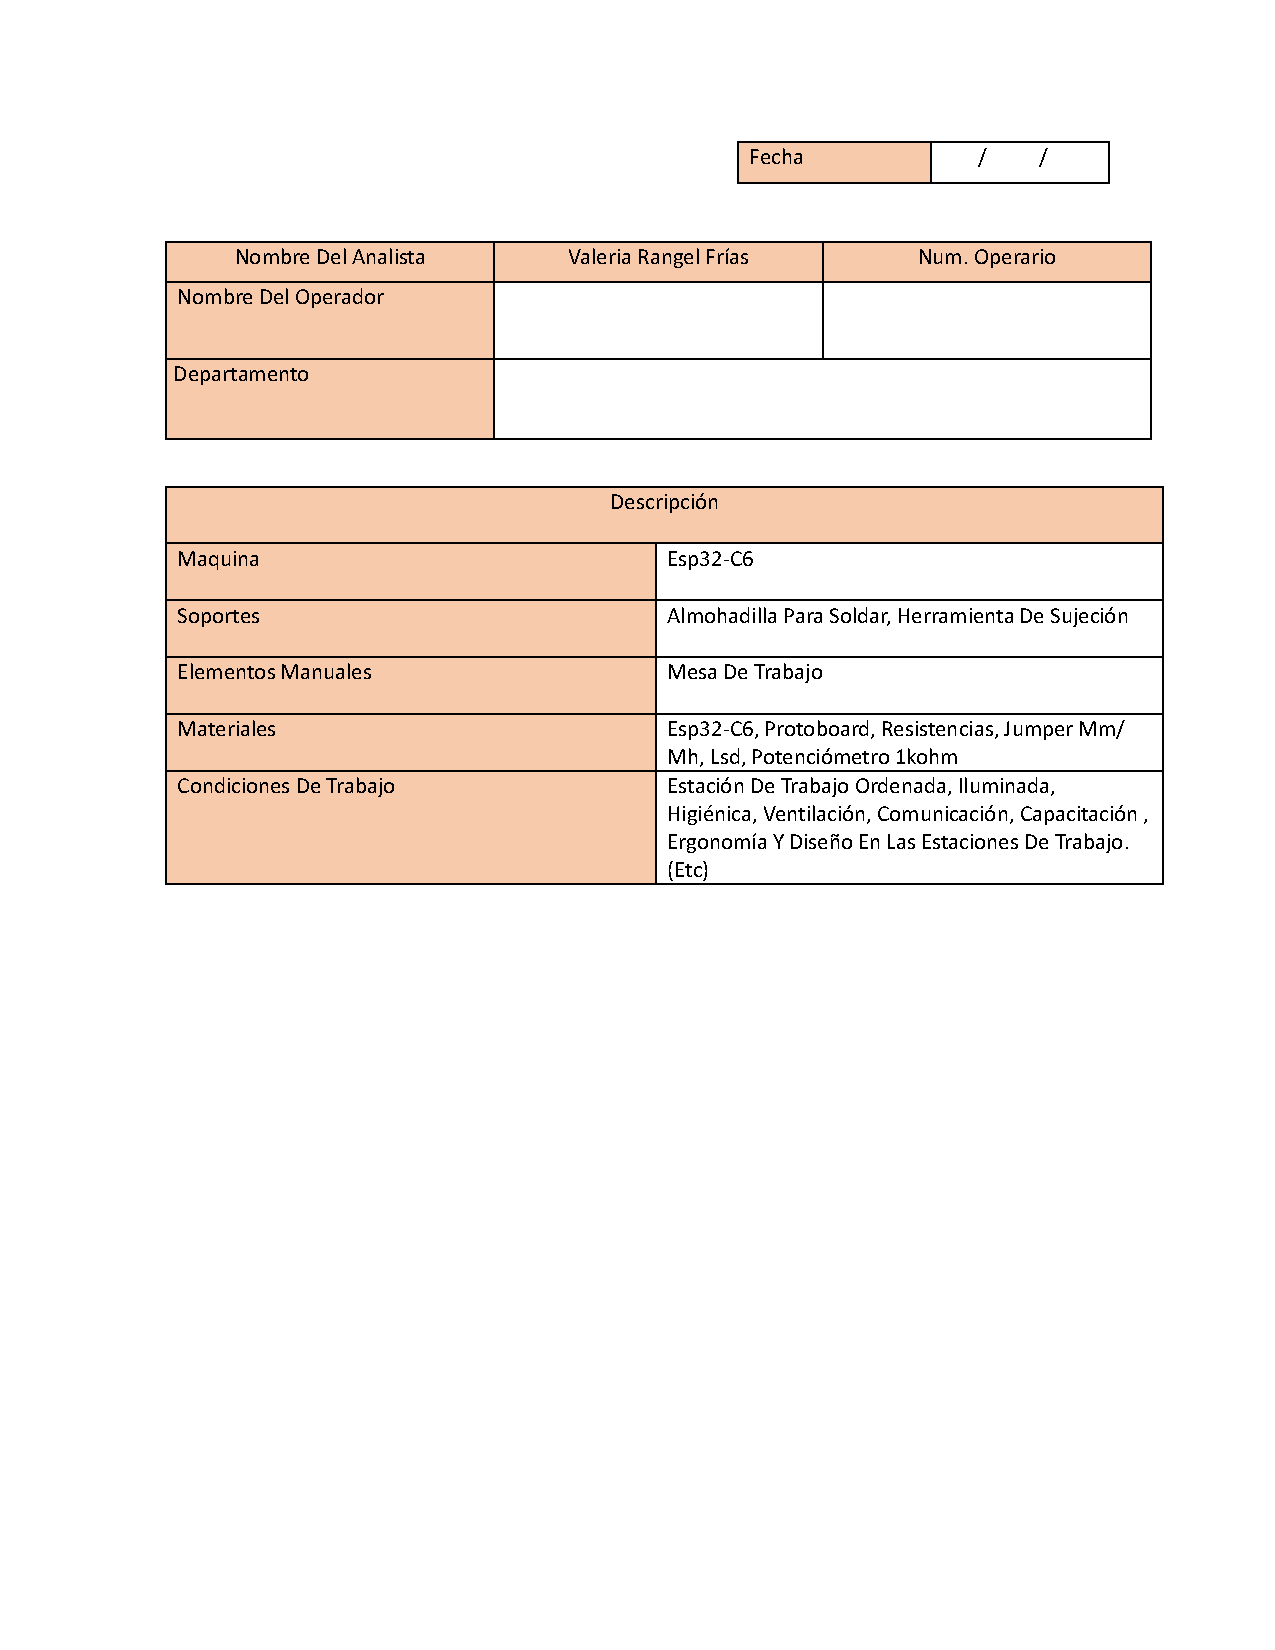
\includepdf[pages=-]{29/img/camelCase.pdf}
    \label{anexo:MANUAL}
    %%%%%%%%%%%%%%%%%%%%%%%%%%%%%%%%%%%%%%%%